\section{Introductie}
\label{sec:intro}
Bij de Tweede Kamerverkiezingen in Nederland kunnen kandidaten met voorkeurstemmen gekozen worden. Hierbij moet een kandidaat een kwart van het aantal stemmen halen dat een partij nodig heeft om één zetel te behalen. Het aantal stemmen dat behaald moet worden voor één zetel wordt de \textit{kiesdeler} genoemd. Het aantal stemmen dat een kandidaat nodig heeft om met voorkeur gekozen te worden wordt de \textit{voorkeursdrempel} genoemd. De voorkeursdrempel is een kwart van de kiesdeler  \citep{Kiesraad_voorkeursdrempel2}.  In de historie van de Tweede Kamerverkiezingen in Nederland is het slechts twaalf maal voorgekomen dat een kandidaat met voorkeurstemmen in de Tweede Kamer is gekozen \citep{Voork74:online}. Bij de Tweede Kamerverkiezingen van 2012 is dit voor het laatst gebeurt. Pieter Omtzigt van het CDA werd toen met voorkeurstemmen gekozen.\

Dit onderzoek is grotendeels gemodelleerd op de Tweede Kamerverkiezingen van 2012. Bij deze verkiezingen werd er voornamelijk op de hoogst genoteerde kandidaten gestemd (zie Figuur \ref{fig:sv2012}). Lager genoteerde kandidaten ontvingen over het algemeen niet genoeg stemmen om boven de voorkeursdrempel uit te komen. Hierdoor zijn, op Pieter Omtzigt na, alle kandidaten op basis van hun plaats op de kandidatenlijst in de Tweede Kamer gekozen. Bij het verdelen van de zetels aan de kandidaten wordt er, conform de kieswet \citeyearpar{kieswetje}, eerst gekeken naar het aantal stemmen die een kandidaat heeft ontvangen. Vervolgens wordt er pas gekeken naar de plaats op de kandidatenlijst. Een kandidaat die aan de voorkeursdrempel voldoet krijgt zodoende de voorkeur boven een kandidaat die hoger genoteerd staat maar niet aan de voorkeursdrempel voldoet. 


\begin{figure}[H]


	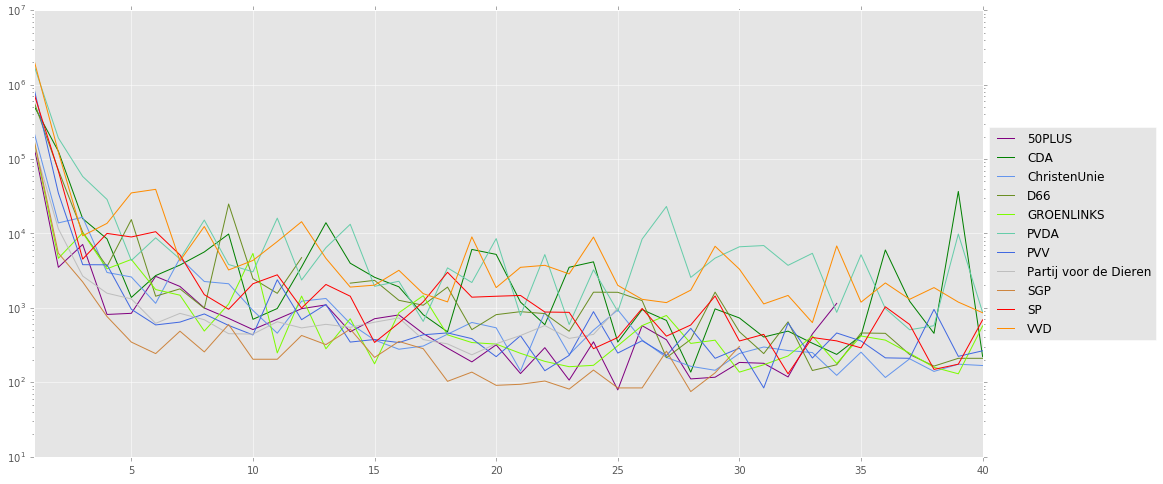
\includegraphics[width=\linewidth]{verdeling_stemmen_2012.png}

			\caption{Per partij de verdeling van de stemmen over de eerste veertig kandidaten bij de Tweede Kamerverkiezingen van 2012 \citep{Kiesraad_databank}. Ten behoeve van de leesbaarheid is er een logaritme over de y-as toegepast.}

\label{fig:sv2012}
\end{figure}

In dit onderzoek zullen we gaan kijken hoe specifieke bevolkingsgroepen de regel van de voorkeursdrempel in hun voordeel kunnen gebruiken om in hogere mate vertegenwoordigd te worden. Deze bevolkingsgroepen zijn:\\

\newcolumntype{L}{@{}>{\bfseries}p{16em}<{}}% Item label
\newcolumntype{I}{X@{}}% Item contents
\noindent\begin{tabularx}{\textwidth}{LI}
Vrouwen: & De stemgerechtigde vrouwen in Nederland. \\
  \\
 Allochtonen: & De stemgerechtigde allochtonen in Nederland. Hierbij wordt de definitie van het CBS  \citeyearpar{Watve22:online} gehanteerd. Volgens het CBS is een persoon een allochtoon wanneer de persoon zelf of één van de ouders van de persoon in het buitenland is geboren. We maken hierbij geen onderscheid tussen westerse en niet-westerse allochtonen.
\\
\end{tabularx}
  
  \newcolumntype{L}{@{}>{\bfseries}p{16em}<{}}% Item label
\newcolumntype{I}{X@{}}% Item contents
\noindent\begin{tabularx}{\textwidth}{LI}

  Ouderen: & De stemgerechtigden personen met een leeftijd van vijftig jaar en ouder. Hierbij worden de definities van de Rijksoverheid \citeyearpar{Wiebe32:online} gecombineerd. Volgens de Rijksoverheid is er geen strike definitie van een oudere. De Rijksoverheid definieert oudere op de arbeidsmarkt als personen van vijftig tot 65 jaar. Bij AOW-gerechtigden gaat het om personen van 65 jaar en ouder. Zodoende combineren we deze twee definities tot één definitie.  \\
\\  
Provincialen: & Voor de provincialen is er geen allesomvattende definitie te vinden. Zodoende hebben we de definitie Randstedelingen gebruikt om personen wonenden in de Randstad te defini\"{e}ren \citep{Rands36:online}. Stemgerechtigde personen niet in de Randstad wonen worden in dit onderzoek aangeduid met provincialen. \\
  \\
\end{tabularx}

In Figuur \ref{fig:az2012} zien we in welke aantallen de bovenstaande bevolkingsgroepen vertegenwoordigd zijn. Aan de hand van data verkregen van het CBS \citeyearpar{CBS_stemgedrag} is onderzocht of de vertegenwoordiging van de bevolkingsgroepen een afspiegeling is van de stemgerechtigden in Nederland ten tijde van de Tweede Kamer verkiezingen in 2012.
De verdeling van het aantal stemgerechtigde vrouwen en mannen in Nederland in 2012 was nagenoeg gelijk met beiden een 50\% aandeel in het aantal stemgerechtigden. Zodoende kunnen we concluderen dat de bevolkingsgroep vrouwen ondervertegenwoordigd is met een aandeel van 38,7\% van de zetels. 
De verdeling stemgerechtigde allochtonen en autochtonen in Nederland in 2012 was grofweg 20\% allochtonen om 80\% autochtonen. Zodoende kunnen we concluderen dat ook de bevolkingsgroep allochtonen ondervertegenwoordigd is met een aandeel van 8,7\% van de zetels. 
De verdeling van het aantal stemgerechtigde ouderen en het aantal stemgerechtigden met een leeftijd van onder de vijftig jaar in Nederland in 2012 was grofweg 49\% ouderen en 51\% stemgerechtigden met een leeftijd van onder de vijftig jaar. Zodoende kunnen we ook voor de bevolkingsgroep ouderen concluderen dat zij met 25.3\% van de zetels ondervertegenwoordigd zijn in de Tweede Kamer. 
De verdeling van het aantal stemgerechtigde provincialen en Randstedelingen was grofweg 67\% provincialen om 33\% Randstedelingen. Zodoende kunnen we ook voor de bevolkingsgroep provincialen concluderen dat zij met 50\% van de zetels ondervertegenwoordigd zijn in de Tweede Kamer. 

\begin{figure}[H]
\centering

	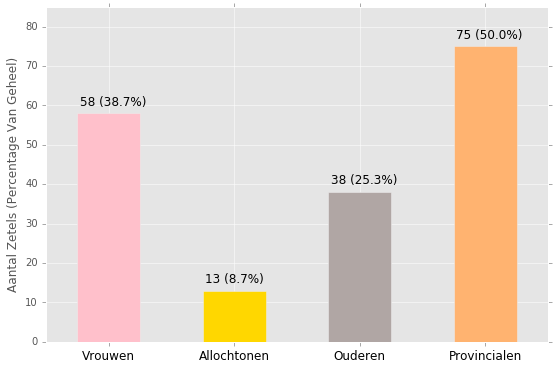
\includegraphics[width=0.55\linewidth]{aantal_zetels_bevolkingsgroepen.png}

			\caption{Het aantal gekozen kamerleden per bevolkingsgroep bij de Tweede Kamerverkiezingen van 2012 \citep{Kiesraad_uitslag}. De groepen zijn allen van een eigen kleur voorzien. Deze kleuren zullen in het gehele paper corresponderen met de respectievelijke bevolkingsgroepen.}

\label{fig:az2012}
\end{figure}

Naast het feit dat de beschreven bevolkingsgroepen ondervertegenwoordigd zijn in de Tweede Kamer na de verkiezingsuitslag van 2012, is uit diverse literatuur op te maken dat het voor de bevolkingsgroepen alsmede voor de politiek en de democratie gunstig is wanneer een parlement aan afspiegeling van de samenleving  \citep{tremblay1998female,anwar2001participation}. Uit een onderzoek van \cite{banducci2004minority} blijkt dat des te beter bevolkingsgroepen als vrouwen en minderheden vertegenwoordigd worden in het parlement, des te positiever er vanuit deze bevolkingsgroepen tegen de politiek aangekeken wordt. Tevens wordt onder deze bevolkingsgroepen de deelname aan parlementsverkiezingen vergroot. Onderzoek van \cite{wangnerud2009women} en \cite{sainsbury2004women} toont aan dat de belangen van vrouwen steeds beter behartigd worden naarmate het aantal vrouwelijke leden in het parlement toeneemt. Volgens \cite{mansbridge1999should} worden vrouwen en negeroïde burgers het beste vertegenwoordigd door respectievelijk vrouwelijk en negeroïde parlementsleden. De reden hiervoor is dat deze parlementsleden bedachtzamer kunnen opereren wanneer het om politieke kwesties gaat die deze leden van de bevolking treffen. Uit een onderzoek van \cite{broockman2014female} blijkt, in tegenstelling tot de verwachting, dat een stijging in het aantal vrouwen dat een politiek ambt bekleedt er niet toe leidt dat er meer vrouwen naar de stembus gaan. Echter heeft het onderzoek enkel betrekking op de Verenigde Staten en wordt geen verder onderzoek verricht naar de toe- of afname van de algehele betrokkenheid van vrouwen voor de politiek en de politieke besluitvorming. In het onderzoek van \cite{karp2008politics} wordt er echter wel geconcludeerd dat betrokkenheid onder vrouwen voor de politiek toeneemt naar mate meer vrouwen zich kandideren voor verkiezingen en naar mate er meer vrouwen een politieke ambt bekleden. 

Naast de effecten die adequatere vertegenwoordiging van bepaalde bevolkingsgroepen met zich meebrengen, blijkt dat vrouwen en minderheden beter vertegenwoordigd zijn in landen waar een evenredige vertegenwoordiging wordt gehanteerd \citep{macivor1999proportional,mcallister2002electoral,studlar1999will,welch1990multi}.  Nederland is een land dat een evenredige vertegenwoordiging hanteert. Dit houdt in dat het percentage stemmen evenredig is met het percentage te ontvangen zetels \citep{Kiess35:online}. Oftewel als een partij 10\% van de stemmen heeft ontvangen krijgt deze partij ook 10\% van de zetels.

Al het voorgaande in ogenschouw nemend wordt er in dit onderzoek onderzocht of er strategie\"{e}n op te stellen zijn onder de leden van de verschillende bevolkingsgroepen waardoor zij adequater vertegenwoordigd kunnen worden in de Tweede Kamer. Binnen dit onderzoek gaan we uit van de meest realistische aannames. Dit houdt in dat we uitgaan van de verdeling van zetels en stemmen over de partijen zoals deze werden voorspeld bij de laatste peiling van 11 september 2012 \citep{IPSOS} en zoals deze daadwerkelijk waren na de verkiezingsuitslag van 2012 \citep{Kiesraad_uitslag}. Aan de hand van de peilingen proberen we strategie\"{e}n op te zetten en aan de hand van de einduitslag zullen we testen hoe succesvol deze strategie\"{e}n zouden zijn geweest. Het doel is om met behulp van deze strategie\"{e}n een maximum aantal leden van een bevolkingsgroep in de Tweede Kamer te krijgen door effectiever gebruikt te maken van de voorkeursdrempel. De hoofdonderzoeksvraag luidt dan ook: \\


\begin{HOV}
\large
"Hoe kunnen specifieke bevolkingsgroepen in Nederland bij de Tweede Kamerverkiezingen de regel van de voorkeursdrempel in de kieswet in hun voordeel benutten?"\\
\end{HOV}

\normalsize
Om tot een antwoord op de bovenstaande hoofdonderzoeksvraag te komen zullen we met het onderzoek verder de diepte in gaan d.m.v. opdeling in deelvragen. Hiervoor hebben zijn vijf deelvragen opgezet en twee subdeelvragen. Aan de hand van de eerste deelvraag zullen we onderzoeken wat het maximum aantal kandidaten per bevolkingsgroep zou zijn geweest wanneer de bevolkingsgroep bepaalde strategie\"{e}n hadden uitgevoerd. De eerste deelvraag luidt daarmee als volgt:\\

\begin{DV}
"Wat is het theoretisch maximum aantal kandidaten dat per specifieke bevolkingsgroep in de Tweede Kamer gekozen had kunnen worden bij de verkiezingen van 2012?"\\\
\end{DV}

Deze eerste deelvraag zal worden beantwoord in Hoofdstuk \ref{sec:eva}. In dit hoofdstuk zullen we vijf verschillende soorten strategie\"{e}n gaan uitrollen en per  bevolkingsgroep gaan toepassen. Aan de hand van de peilingen proberen we eerst een voorspelling te doen hoe de stemmen verdeeld zullen worden wanneer 100\% van de bevolkingsgroep zich committeert aan een strategie. Vervolgens zullen we in het daaropvolgende hoofdstuk gaan onderzoeken welke factoren er van invloed kunnen zijn op het behalen van het maximum aantal kandidaten per bevolkingsgroep. De tweede deelvraag luidt daarom: \\

\begin{DV}" Welke factoren kunnen per bevolkingsgroep van invloed zijn op het wel of niet behalen van het theoretisch maximum aantal kandidaten dat in de Tweede Kamer gekozen kan worden?"\\\
\end{DV}

Nadat de factoren en hun invloed zijn beschreven, wordt er onderzocht welke strate\"{e}n aan te bevelen zijn richting de bevolkingsgroepen. De derde deelvraag luidt:\\

\begin{DV}"Welke strategie is per specifieke bevolkingsgroep aan te bevelen wanneer zij de regel van van voorkeursdrempel in de kieswet in hun voordeel willen benutten?"\\\
\end{DV}

Vanwege de verleiding te kiezen voor een strategie die in Hoofdstuk \ref{sec:eva} zich bewezen heeft als de strategie met het hoogste rendement kan men geneigd zijn de complexiteit van een strategie over het hoofd te zien als het gaat om de wijze van uitvoering. Vandaar dat dit onderzoek bij deze deelvraag niet poogt om een direct antwoord te hierop te verschaffen maar zal er verder de diepte ingegaan worden om daarmee te onderzoeken hoe de strategie\"{e}n uit te voeren zijn. Derhalve wordt de derde deelvraag verder opgedeeld in twee subdeelvragen. De eerste subdeelvraag luidt:\\

\begin{SDV}"Hoe kan een strategie uitvoerbaar worden gemaakt voor een specifieke bevolkingsgroep waarvan de leden zich willen committeren aan een strategie om de regel van de voorkeursdrempel in hun voordeel te benutten?"\\\
\end{SDV}

Met het beantwoorden van deze subdeelvraag zullen we een tweetal van hulpmiddelen voorstellen in de vorm van IT-toepassingen. Tevens stellen we ook een derde hulpmiddel voor. Dit derde hulpmiddel is een mengvorm van de eerste twee hulpmiddelen. Deze hulpmiddelen zullen slechts dienen als voorbeelden en verder onderzoek zal hierbij ook nodig zijn wanneer deze toepassingen daadwerkelijk worden ontwikkeld. Echter zullen we al wel ingaan op enkel voor- en nadelen die deze hulpmiddelen met zich mee kunnen brengen. Tevens zullen we de voor- en nadelen onderzoeken die kunnen ontstaan wanneer er geen hulpmiddelen worden ingeschakeld. Zodoende luidt de tweede subdeelvraag als volgt: \\\

\begin{SDV}"Wat zijn de eventuele voor- en nadelen van de keuze van de wijze waarop een strategie zal worden uitgevoerd?"\\\
\end{SDV}

Nadat a.d.h.v. de eerste deelvraag is onderzocht met welke strategie\"{e}n het maximum aantal vertegenwoordigers van een bevolkingsgroep in de Tweede Kamer gekozen hadden kunnen worden, wordt in Hoofdstuk \ref{h7} onderzocht wat er kan gebeuren wanneer leden van een andere bevolkingsgroep (of bevolkingsgroepen) zich committeert aan een tegenstrategie. Hierbij zullen we onderzoeken of er een toestand bereikt kan worden waarin beiden (of meerdere) bevolkingsgroepen een strategie hanteren en er een Nash Equilibrium onstaat. Hierbij luidt de vierde deelvraag: \\\

\begin{DV}"Wat kan er gebeuren wanneer een bevolkingsgroep zich committeert aan een strategie en een andere bevolkingsgroep zich committeert aan een tegenstrategie?"\\\
\end{DV}

Tot slot zal er een advies worden uitgebracht betreffende het voorkomen van uitbuiting van de voorkeursdrempel. Hierbij kunnen twee (of meerdere) bevolkingsgroepen een strategie uitvoeren maar geen van beide bevolkingsgroepen kan daarbij de regel van de voorkeursdrempel in haar/zijn eigen voordeel op zo een manier weten uit te buiten dat het d.m.v. het uitvoeren van een strategie oververtegenwoordigd zal zijn. Oftewel we adviseren een aanpassing van de kieswet wat er voor moet zorgen dat er geen overmatig misbruik van de regel van de voorkeursdrempel mogelijk zal zijn. De laatste deelvraag luidt daarom: \\\

\begin{DV}" Hoe kan er voorkomen worden dat de voorkeursdrempel in het voordeel van een bevolkingsgroep kan worden uitgebuit?"\\\
\end{DV}

Nadat de deelvragen zo adequaat mogelijk zijn beantwoord, zal er een conclusie getrokken worden en een aantal aanbevelingen gedaan worden op basis van bevindingen in het onderzoek. 






\iffalse
\begin{itemize}
\item Bevat je onderzoeksvraag (of vragen)
\item Plaatst je vraag in de bestaande literatuur.
\end{itemize}

Je onderzoeksvraag is leidend voor je hele scriptie. Alles wat je doet moet uiteindelijk terug te voeren zijn op 1 doel: het beantwoorden van die vraag. 

Typisch zal je het dan ook zo doen:

Mijn onderzoeksvraag is onderverdeeld in de volgende deelvragen:

\begin{description}
\item[RQ1] \ldots We   beantwoorden deze vraag  door het volgende te doen/ antwoord op de volgende vragen te vinden/ \ldots
\begin{enumerate}
\item Vragen op dit niveau kan je echt beantwoorden, en dat doe je in je Evaluatie sectie~\ref{sec:eva}.
\end{enumerate}
\item[RQ2] \ldots
\item[RQ3] \ldots
\end{description}

Je Evaluatie sectie~\ref{sec:eva} bevat evenveel subsecties als je deelvragen hebt. En in elke sectie beantwoord je dan die deelvraag met behulp van de vragen op het onderste niveau.

In je conclusies kan je dan je hoofdvraag gaan beantwoorden op basis van al het eerder vergaarde bewijs.


\paragraph{Overview of thesis}
Hier geef je even kort weer wat in elke sectie staat.
\fi



\newpage